\documentclass{article}

\usepackage[a4paper, margin=1in]{geometry}
\usepackage[onehalfspacing]{setspace} % Correct 1.5 line spacing

\usepackage{graphicx}  % Figures
\graphicspath{{../figures/}}

\usepackage{url}
\usepackage[pdfusetitle]{hyperref}
\usepackage{titlesec}      % Modify title/section/chapter commands
\usepackage{mathtools}     % Various maths related commands
\usepackage{gensymb}       % \degree symbol
\usepackage[thinc]{esdiff} % Derivatives
\usepackage{booktabs}      % \toprule, etc., in tables
\usepackage{doi}           % support DOI links in bibliography
\usepackage{wrapfig}       % figures in text

\usepackage{fontspec}  % Fonts
\usepackage{helvet}
\usepackage{newpxtext,newpxmath}
\defaultfontfeatures{Scale=MatchLowercase, Ligatures=TeX}

% SI units
\usepackage{siunitx}
\sisetup{separate-uncertainty=true,number-mode=text,detect-weight=true}
\DeclareSIUnit\belm{Bm}
\DeclareSIUnit\belw{BW}
\DeclareSIUnit\beli{Bi}
\DeclareSIUnit\belz{BZ}

% https://tex.stackexchange.com/a/43009
\DeclarePairedDelimiter\abs{\lvert}{\rvert}%
\DeclarePairedDelimiter\norm{\lVert}{\rVert}%

% Caption figures
\usepackage{caption}
\DeclareCaptionFont{captionlabelfont}{\bfseries \sffamily}
\DeclareCaptionFont{captiontextfont}{\sffamily}
\captionsetup{labelfont=captionlabelfont, textfont=captiontextfont}

% Change footnote style
\renewcommand{\thefootnote}{\fnsymbol{footnote}}

% Fancy header/footer
\usepackage{fancyhdr}
\pagestyle{fancy}
\renewcommand{\sectionmark}[1]{\markright{\thesection . #1}}
\fancyhf{}
\lhead{\fancyplain{}{\thepage}}
\rhead{\fancyplain{}{\textit{\rightmark}}}

% Bibliography
\usepackage[backend=biber, style=ieee, natbib=true,
			url=false, isbn=true, doi=true,
			eprint=false, urldate=long]{biblatex}
\addbibresource{references.bib}

% biblatex IEEE style leaves empty parentheses when there is no date/year field.
% Since there are no date fields for many online resources, we use
%   https://tex.stackexchange.com/a/151264
% to stop these parentheses from being generated if there is no date field.
\usepackage{xpatch}
\xpatchbibdriver{online}
{\printtext[parens]{\usebibmacro{date}}}
{\iffieldundef{year}
	{}
	{\printtext[parens]{\usebibmacro{date}}}}
{}
{\typeout{There was an error patching biblatex-ieee (specifically, ieee.bbx's @online driver)}}

% Fix for missing µ in siunitx ???
% https://tex.stackexchange.com/a/428215
\sisetup{math-micro=\text{µ},text-micro=µ}

\newcommand\mytitle    {Millimetre-Wave Cloud Profiling Radar}
\newcommand\mysubtitle {Pre-Project Review}
\newcommand\myauthor   {180014855}
\newcommand\mydate     {\today}
\newcommand\mymodule   {PH4111}
\newcommand\mywordcount{2300}

\title {\mytitle}
\author{\myauthor}
\date  {\mydate}

\begin{document}

\begin{titlepage}
	\centering
	{
\includegraphics[width=0.3\textwidth]{uos-logo}}
	\par
	{\LARGE\bfseries University of St Andrews\par}
	{\LARGE School of Physics and Astronomy\par}
	\vspace{1.5cm}
	{\huge\bfseries\mytitle\par}
	{\Large\mysubtitle\par}
	\vspace{2cm}
	{\Large\myauthor\par}
	{\large\textbf{Module:} \mymodule\par}
	{\large\textbf{Word count:} \mywordcount\par}
	\vfill
	{\large\today\par}
\end{titlepage}

\section{Introduction}
\begin{figure}
	\centering
	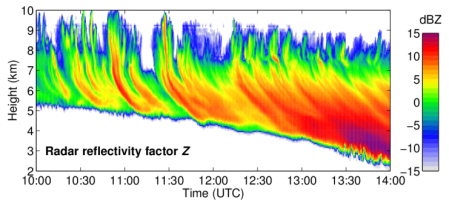
\includegraphics[width=\textwidth]{example-output}
	\caption{Example range-time plot from a cloud profiling radar.\supercite{RPG}}
	\label{fig:ExampleOutput}
\end{figure}
Meteorological radar systems provide great insight into weather phenomena, allowing for improved forecasts and for meteorologists to study clouds on a large scale. Clouds have a great influence on Earth’s surface temperature, being able to both reflect and trap solar radiation, thus it is essential to study clouds to accurately model climate change. However, the high cost of conventional pulse-Doppler radars limits their deployment and hence the amount of cloud data that can be gathered.\supercite{Illingworth} Much attention has been devoted to frequency-modulated continuous wave (FMCW) radars which require significantly less power and so less expensive amplifiers can be used. FMCW radars generally offer better range resolution compared to pulse-Doppler systems.

Millimetre waves are particularly suitable for cloud radars due to having high reflectivity to small particles such as cloud droplets (\(0.01\) to \SI{0.1}{\milli\metre})\supercite{FirstCourse} whilst still penetrating cloud layers. However, at millimetre wavelengths attenuation from the atmosphere is a significant problem.\supercite{KolliasFrontier} For this reason most cloud radars operate near local minima in the absorption spectrum (Fig. \ref{fig:Attenuation}), usually \SI{35}{\giga\hertz} or \SI{94}{\giga\hertz}. Higher frequencies are preferred for cloud radars due to increased radar cross-section (RCS) for smaller particles (Fig. \ref{fig:RayleighCurve}). At wavelengths close to particle diameter, the RCS begins to taper off and becomes more accurately described by Mie scattering theory,\supercite{POMRRayleighScattering} which complicates calculations.

\begin{figure}
	\centering
	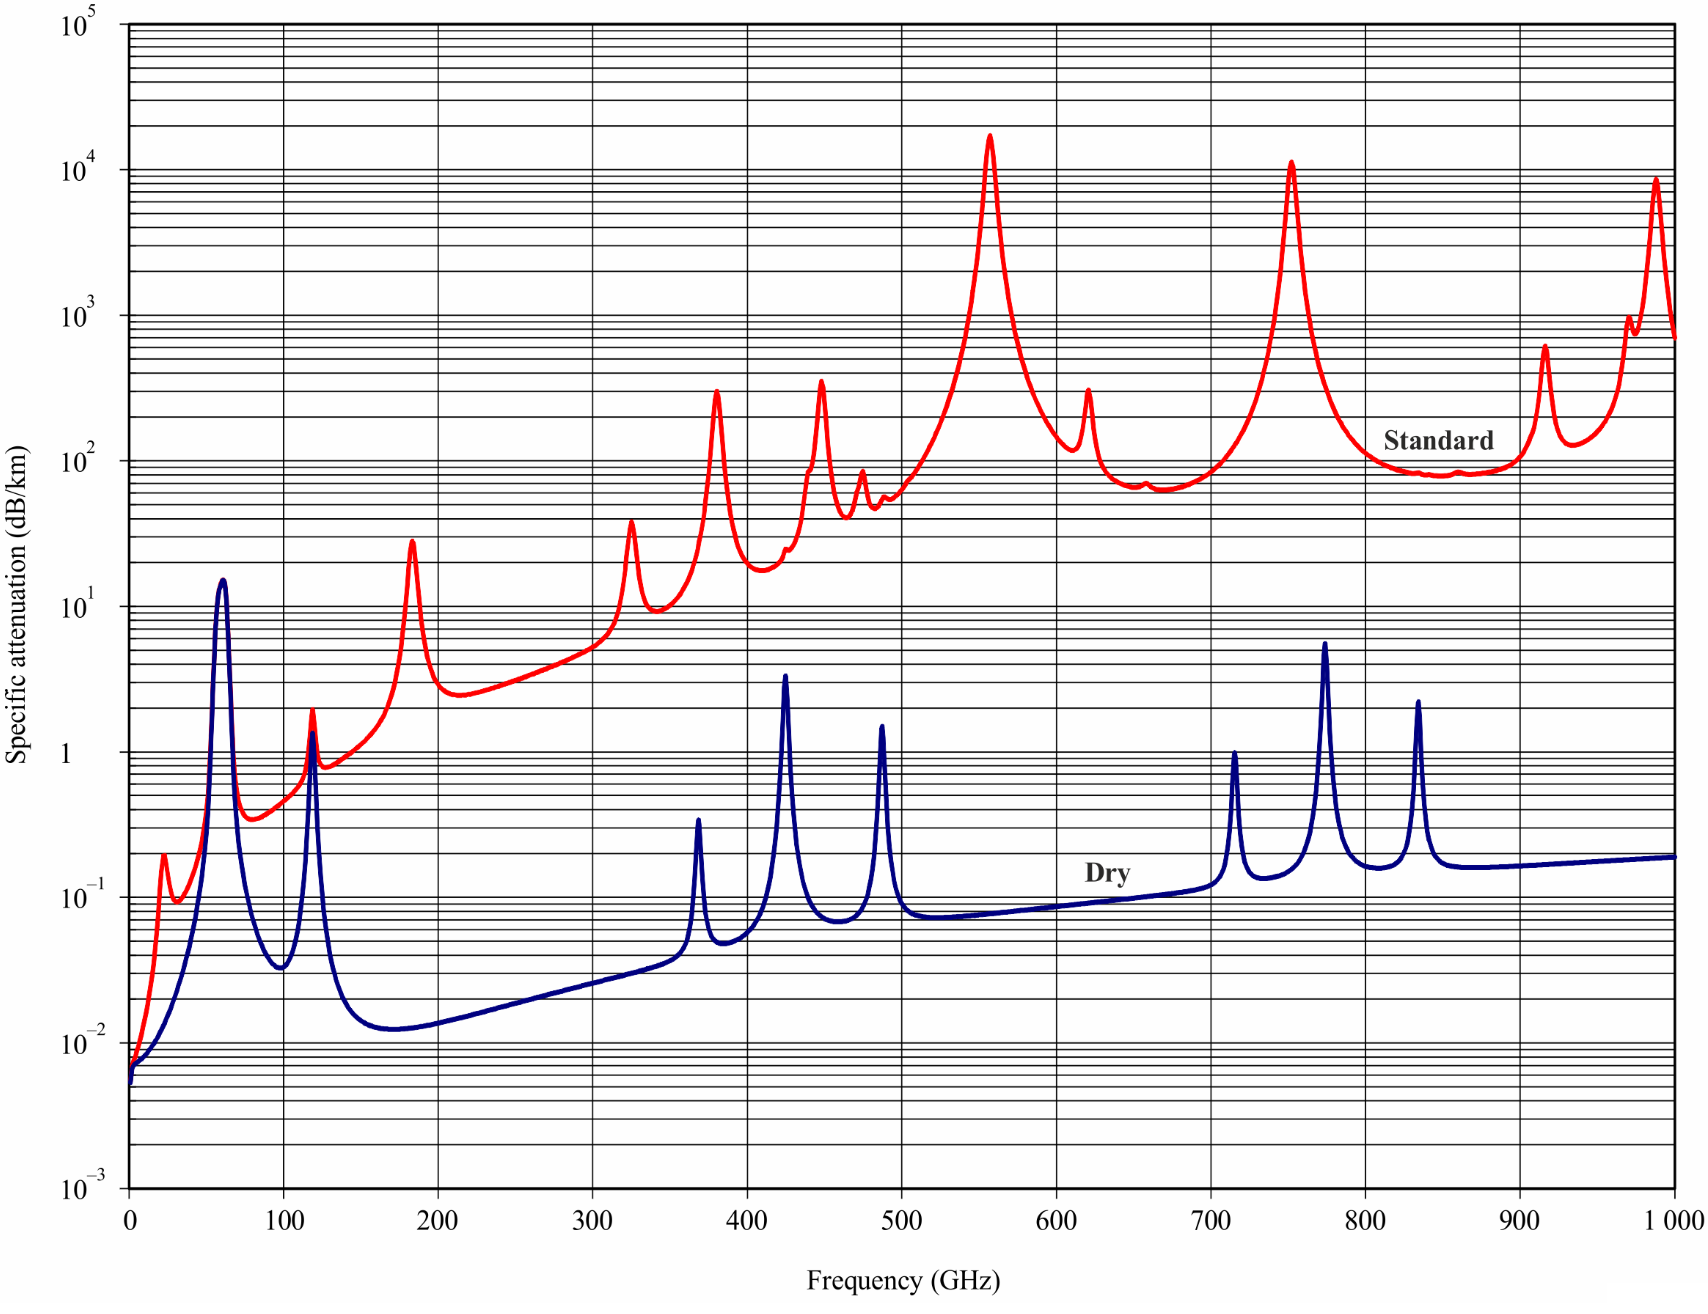
\includegraphics[width=0.8\textwidth]{attenuation}
	\caption{Atmospheric attenuation as a function of radar frequency for dry and standard atmosphere conditions.\supercite{ITURAttenuation} Peaks corresponding to absorption by molecules in the atmosphere are visible throughout.}
	\label{fig:Attenuation}
\end{figure}
\begin{figure}
	\centering
	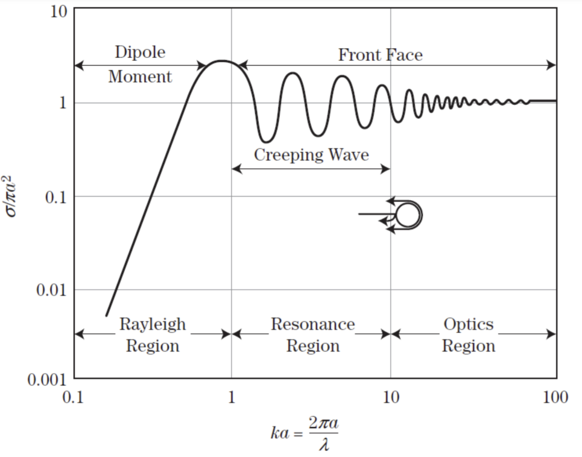
\includegraphics[width=0.8\textwidth]{rayleigh}
	\caption{Radar cross-section of spherical particles as a function of radius and wavelength. The Rayleigh backscattering approximation is only applicable in the linear regime, where the particle size is small relative to the wavelength. As the ratio between particle size and wavelength increases, the behaviour is more accurately described by Mie theory.\supercite{POMRRayleighScattering}}
	\label{fig:RayleighCurve}
\end{figure}

\section{Frequency-modulated continuous wave radar}
FMCW radar systems emit consecutive 'chirps' - signals whose frequency is linearly modulated by triangular or more commonly sawtooth The reflected chirp arrives at a time \(\Delta t\) after emission, leading to a phase difference as shown in Fig. \ref{fig:Chirp}. The transmitted and received signals are passed through a mixer to extract their difference/intermediate frequency (IF) on which some signal processing can be performed to determine the range and velocity.

\begin{figure}[h!]
	\centering
	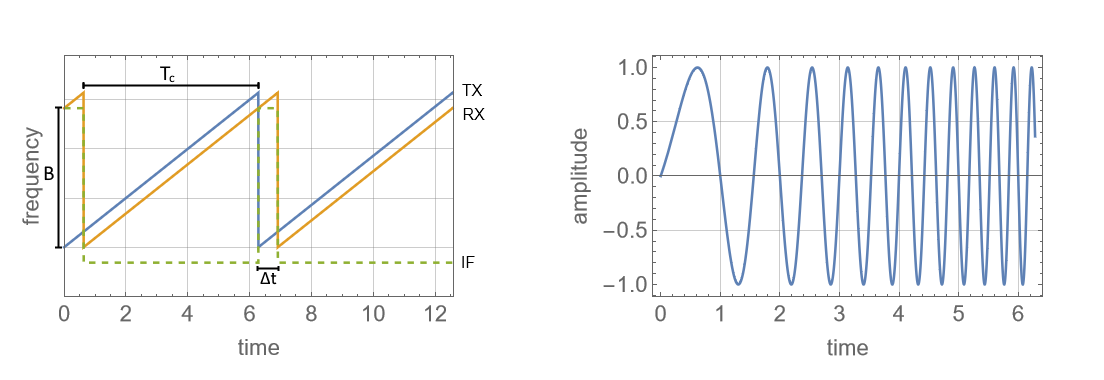
\includegraphics[width=\textwidth]{chirp-3}
	\caption{Left: transmitted (TX) and received (RX) sawtooth chirps and their difference frequency (IF). Right: illustration of TX chirp waveform. (Own work)}
	\label{fig:Chirp}
\end{figure}

\paragraph{Range measurement.} The target range relates to the time delay and hence the intermediate frequency \(f_{IF}\) by
\begin{equation}
	r = \frac{c \Delta t}{2} = \frac{c f_{IF} T_c}{2 B},
\end{equation}
where \(r\) is the distance from the radar and \(T_c\) is the chirp duration.\supercite{TIFMCWDoppler}
In practice, there are many received signals, thus one performs a discrete Fourier transform of the IF signal to obtain a range profile, known as a range-FFT. Since the range-FFT is discrete, the range resolution is limited by the bandwidth \(B\) of the chirp:
\begin{equation}
	r_{res} = \frac{c}{2B}.
\end{equation}

\paragraph{Velocity measurement.} Two targets at roughly the same range appear in the same bin on the range-FFT. Fortunately, it is possible to distinguish them by considering the phase of the signal in each bin across subsequent chirps. If a target is moving at a velocity \(v\), the phase of the IF signal changes by an amount given by\supercite{TIFMCWDoppler}
\begin{equation}
	\delta = \frac{4 \pi v T_c}{\lambda},
\end{equation}
where \(v\) is the target velocity. The velocity is unambigious only if \(-\pi \le \delta \le \pi\), thus leading to a maximum velocity of
\begin{equation}
	v_{max} = \frac{\lambda}{4 T_c}.
\end{equation}
If the velocity is outwith the interval \([-v_{max}, v_{max}]\), it will 'fold' back in on itself (aliasing).

For multiple targets, we once again perform an FFT (Doppler-FFT)\supercite{POMRDopplerProcessing} on each range bin over a sequence of chirps known as a frame. This imposes a velocity resolution given by
\begin{equation}
	v_{res} = \frac{\lambda}{2 T_f},
\end{equation}
where \(T_f\) is the time per frame.

\section{Meteorological radar theory}
The range equation for a point target is given by
\begin{equation}
	P_r = \frac{P_t G_t G_r \lambda^2}{(4 \pi)^3 r^4} \sigma, \label{eqn:PointTarget}
\end{equation}
where \(P_t\) and \(P_r\) are the transmitter and receiver powers, \(G_t\) and \(G_r\) are transmitter and receiver antenna gains, and \(\sigma\) is the radar cross-section. For distributed targets,
\begin{equation}
	\sigma = V \eta,
\end{equation}
where \(V\) is the radar sample volume and \(\eta\) is the volume reflectivity.

It can be seen from Fig. \ref{fig:Volume} that
\begin{equation}
	V = \frac{1}{8} \pi r^2 \theta \phi \Delta R,
\end{equation}
where \(\theta\) and \(\phi\) are the angular beamwidths, measured from the centre to the \(-\SI{3}{\decibel}\) point of the main lobe. The depth of the range cell \(\Delta R = c\tau\) is given by the pulse width \(\tau\) for pulsed radars, or for FMCW radar \(\tau\) is the reciprocal of the chirp bandwidth \(B\).\supercite{Gorka}

\begin{figure}[h!]
	\centering
	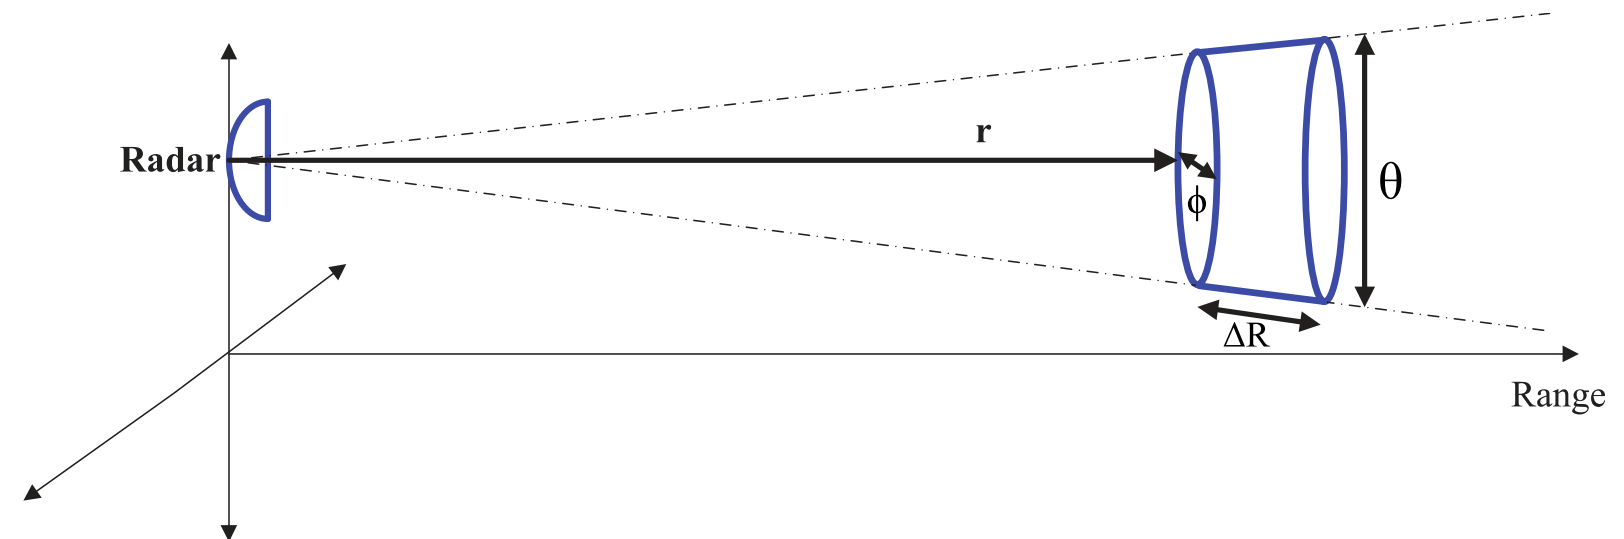
\includegraphics[width=0.8\textwidth]{volume}
	\caption{Diagram of radar sample volume.\supercite{Gorka}}
	\label{fig:Volume}
\end{figure}

The volume reflectivity is essentially the sum of the radar cross-sections for each target per unit volume. Under the Rayleigh backscattering approximation, it takes the form\supercite{FirstCourse}
\begin{equation}
	\eta = \frac{1}{V}\sum_i{\sigma_i} = \frac{\pi^5}{\lambda^4} \abs{K}^2 \frac{\sum_i{D_i^6}}{V} = \frac{\pi^5}{\lambda^4} \abs{K}^2 Z,
\end{equation}
where \(Z\) is the radar reflectivity factor and \(K\) is a constant dependent on phase (water, ice), temperature, and frequency. \(Z\) is by far the most important term since it is independent of radar parameters and can be used to determine cloud types and precipitation intensity. Since values for \(Z\) span many orders of magnitude, it is often expressed on a logarithmic scale \(dBZ\).

Combining the expressions for \(V\) and \(\eta\) yields the range equation for meteorological targets,\supercite{RadarHandbookMeteo}
\begin{equation}
	P_r = \frac{P_t G_t G_r \lambda^2}{(4 \pi)^3 r^4} \cdot \frac{1}{2\ln{2}} \cdot \frac{\pi r^2 \theta \phi c \tau}{8} \cdot \eta = \frac{P_t G_t G_r \lambda^2 \theta \phi c \tau}{1024 (\ln{2}) \pi^2 r^2} \eta = \frac{P_t G_t G_r \theta \phi c \tau \pi^3 \abs{K}^2}{1024 (\ln{2}) \lambda^2 r^2} Z,
	\label{eqn:MeteoRange}
\end{equation}
where we have inserted a factor of \(1/(2\ln{2})\) as suggested by Probert-Jones (1962)\supercite{ProbertJones} to account for the fact that antenna gain is not uniformly distributed across the sample volume.

\subsection{Radar output}
The radar reflectivity factor combined with the range information can be used to identify clouds and estimate precipitation intensity. Fig. \ref{fig:ExampleOutput} is a range-time plot with reflectivity on a logarithmic colour scale.

Just as important is the Doppler velocity spectra and its moments (mean, width, skew, kurtosis) which provides information on microphysical processes in clouds. These moments are of particular interest to meteorologists who wish to study the onset of cloud formation or precipitation, for example.
Fig. \ref{fig:ExampleDopplerSpectra} shows three Doppler spectra taken at different altitudes in a precipitating cloud, showing how the distribution changes as one moves through the melting layer.

Further processing can allow one to determine particle size distribution.\supercite{DopplerMoments}

\begin{table}
	\centering
	\begin{tabular}{l|l}
		Reflectivity factor (dBZ) & Types and approximate base altitudes \\
		\midrule
		less than \(-50\)         & Cumulus (\(0.3\) to \(1.5\) \si{\kilo\metre}), altocumulus (\(2\) to \(6\) \si{\kilo\metre}), thin cirrus (\(6\) to \(12\) \si{\kilo\metre}) \\
		\(-40\) to \(-20\)        & Stratus (\(0\) to \(1.2\) \si{\kilo\metre}), altostratus (\(3\) to \(6\) \si{\kilo\metre}), thick cirrus (\(6\) to \(12\) \si{\kilo\metre})  \\
		\(-20\) and above         & Precipitation
	\end{tabular}
	\caption{Reflectivity factors and associated cloud types,\supercite{KolliasFrontier} including base altitudes.\supercite{CloudTypes}.}
	\label{tbl:dBZInterpretation}
\end{table}

\begin{figure}[h!]
	\centering
	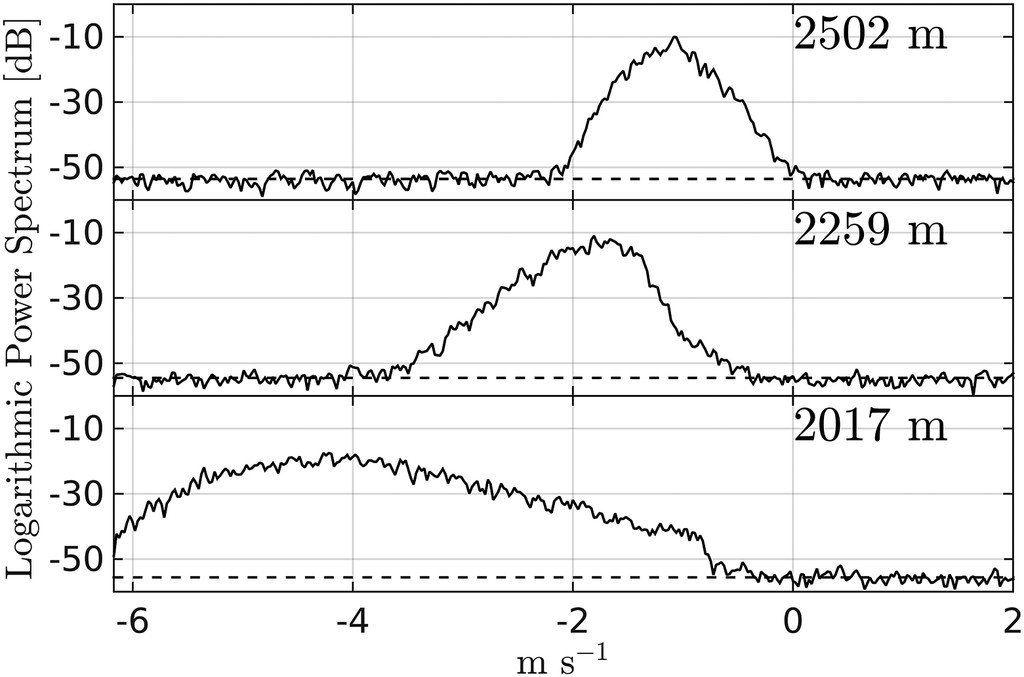
\includegraphics[width=0.6\textwidth]{doppler-spectra}
	\caption{Doppler velocity spectra above (top), within (middle), below (bottom) the melting layer of a precipitating cloud.\supercite{RPGPaper} Above the melting layer, the distribution is roughly Gaussian. Within the layer, the distribution is skewed and the mean velocity increases in magnitude, indicating the acceleration of ice particles as they melt. Below the layer, there is significant broadening of the velocity spectra.}
	\label{fig:ExampleDopplerSpectra}
\end{figure}

\subsection{Radar sensitivity}
Eqn. \ref{eqn:MeteoRange} is more useful if one writes it as a function of the signal-to-noise ratio (SNR) and the thermal noise power by substituting
\begin{equation}
	P_r = SNR \cdot P_n = SNR \cdot k_B T F B_r,
	\label{eqn:SNR}
\end{equation}
where \(P_n\) is the thermal noise power, \(k_B\) is Boltzmann's constant, \(F\) is the noise figure (in linear units), \(T\) is the system temperature, and \(B_r\) is the receiver bandwidth.\supercite{RadarHandbookMeteo}
Eqn. \ref{eqn:SNR} can be used with a minimum desired SNR to obtain the minimum detectable reflectivity (sensitivity) for a given radar. Most clouds have altitudes between \(0\) to \(\SI{12}{\kilo\metre}\) and a radar reflectivity factor between \(-40\) and \(-\SI{20}{\deci\belz}\)\supercite{Gorka} (Table \ref{tbl:dBZInterpretation}).
Sensitivity curves for the radars in Table \ref{tbl:RadarSystems} are given in Fig. \ref{fig:Sensitivity}.

\section{Radar systems}
\subsection{St Andrews \SI{94}{\giga\hertz} FMCW radar}
\begin{figure}
	\centering
	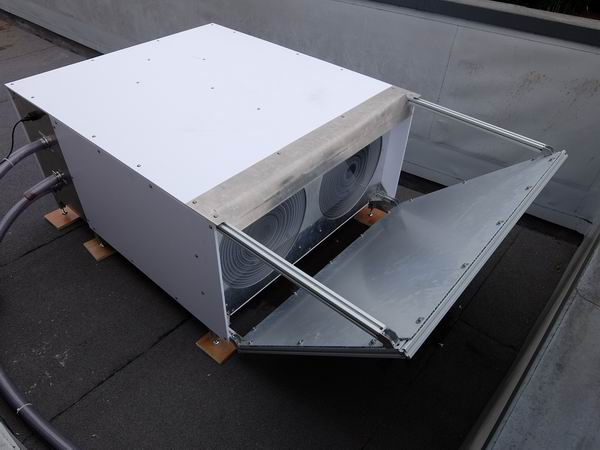
\includegraphics[width=0.6\textwidth]{cloud-radar}
	\caption{St Andrews cloud profiling radar.\supercite{StAndrewsRadarImage}}
	\label{fig:RadarImage}
\end{figure}

\begin{figure}
	\centering
	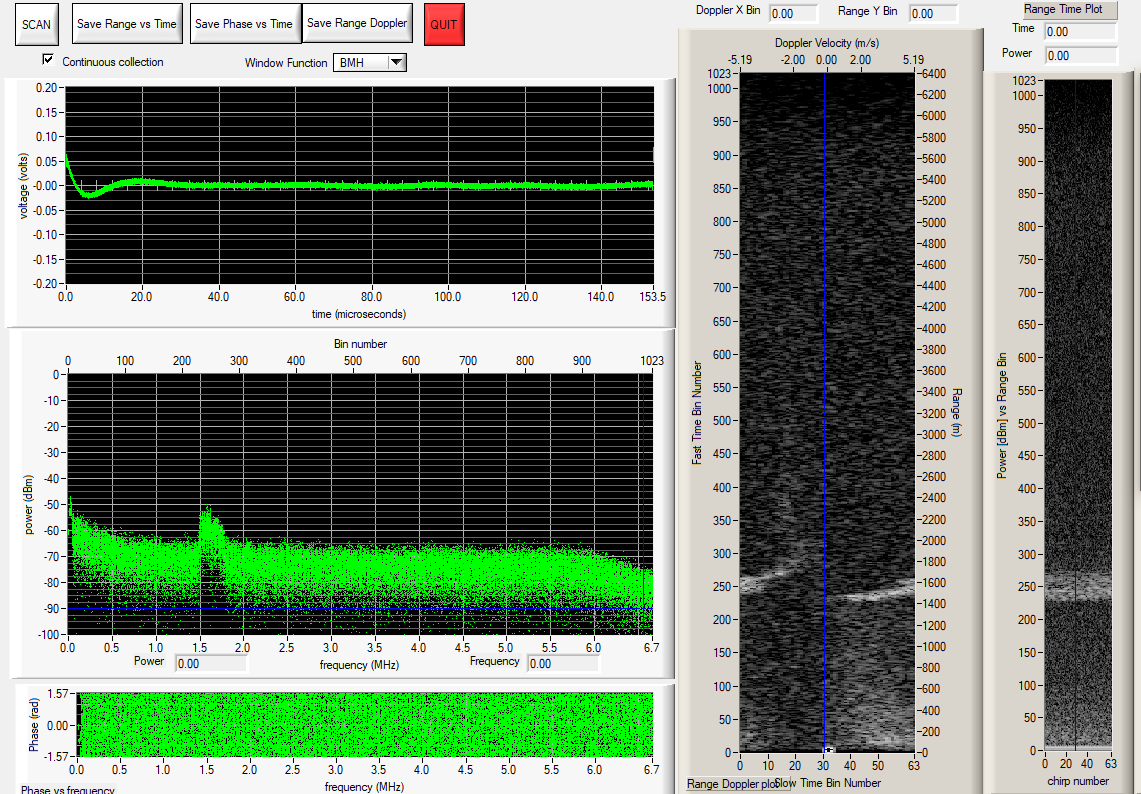
\includegraphics[width=0.8\textwidth]{gui}
	\caption{Screenshot of the St Andrews cloud profiling radar user interface.\supercite{StAndrewsRadar} The peak in the frequency spectrum indicates rain. Aliasing is apparent in the range-Doppler plot at around \SI{1500}{\metre}, as the rain exceeds the maximum unambiguous velocity. Note that the radar is currently uncalibrated.}
	\label{fig:GUI}
\end{figure}

The Millimetre Wave and EPR Group at the University of St Andrews has been developing a ground-based, zenith-pointing radar that operates at \SI{94}{\giga\hertz}.\supercite{StAndrewsRadar} The radar utilises solid-state electronics and two Fresnel zone plate antennas, significantly reducing the cost.
Since FMCW radar requires thousands of FFTs to be performed, the radar software is written in C and leverages multiple CPU threads for best performance. Multithreading comes at the cost of increased software complexity.\supercite{Cassidy}
The sensitivity at \SI{2}{\kilo\metre} is only \(-\SI{20}{\deci\belz}\), just bordering on the range of interest for clouds (\(< -\SI{20}{\deci\belz}\)). However, the sensitivity can be greatly improved by implementing signal averaging as shown in Fig. \ref{fig:Sensitivity}. With \SI{1}{\second} non-coherent averaging,\supercite{POMRNonCoherentAveraging} the sensitivity at \SI{2}{\kilo\metre} is improved to about \(-\SI{-38}{\deci\belz}\).

\subsection{Bistatic Radar System for Atmospheric Studies (BASTA) \SI{95}{\giga\hertz} FMCW cloud radar}
In contrast the CPU-based design of the St Andrews cloud profiling radar, the BASTA\supercite{BASTA} radar implements signal processing using field-programmable gate arrays (FPGA) for improved performance. However, implementing hardware-based signal processing makes it more difficult to debug and reduces the overall flexibility.\supercite{Cassidy}

\subsection{Galileo \SI{94}{\giga\hertz} pulse-Doppler radar}
The Galileo radar\supercite{Galileo} at the Chibolton Observatory is a state of the art pulse-Doppler radar that operates at \SI{94}{\giga\hertz}. While the radar offers better sensitivity than most radars in Table \ref{tbl:RadarSystems}, the peak power requirement (\SI{1.5}{\kilo\watt}) and the range resolution (\SI{75}{\metre}) are significantly greater.

\subsection{Chiba \SI{95}{\giga\hertz} FMCW radar}
Since 2003, Chiba University has been operating a \SI{94.7}{\giga\hertz} FMCW cloud radar\supercite{Chiba} that provides sensitivity on par with the Galileo radar. The antennas have narrower beamwidths (\(0.18\degree\)) than most of the other radars (\(0.4\) to \(0.5\degree\)) except Huggard (\(0.15\degree\)).

\begin{table}
	\begin{tabular}{lr|l|l|l|l|l}
		& & St Andrews\supercite{StAndrewsRadar} & BASTA\supercite{BASTA} & Chiba\supercite{Chiba} & Huggard\supercite{HuggardRadar} & Galileo\supercite{Galileo} \\
		\midrule
		\textbf{Type}                    &                                            & FMCW     & FMCW     & FMCW     & FMCW     & Pulse    \\
		\textbf{Frequency}               & (\si{\giga\hertz})                         & \(94\)   & \(95\)   & \(94.7\) & \(94\)   & \(94\)   \\
		\textbf{Chirp/pulse rep. freq.}  & (\si{\hertz})                              & \(6510\) & \(6250\) & \(1000\) & \(1299\) & \(6250\) \\
		\textbf{Bandwidth / pulse width} & (\si{\mega\hertz} / \(\upmu\si{\second})\) & \(15\)   & \(6\)    & \(10\)   & \(5\)    & \(0.5\)  \\
		\textbf{Range resolution}        & (\si{\metre})                              & \(10\)   & \(25\)   & \(15\)   & \(30\)   & \(75\)   \\
		
		\textbf{Transmit power}          & (\si{\deci\belm})                          & \(25\)   & \(30\)   & \(27\)   & \(23\)   & \(61.8\) \\
		\textbf{Antenna gain}            & (\si{\deci\beli})                          & \(52\)   & \(54\)   & \(57\)   & \(55\)   & \(50\)   \\
		\textbf{Beamwidth}               & (\degree)                                  & \(0.43\) & \(0.4\)  & \(0.18\) & \(0.15\) & \(0.5\)  \\
		
		\textbf{Noise figure}            & (\si{\deci\bel})                           & \(5.3\)  & \(8\)    & \(5.5\)  & \(5\)    & \(9\)    \\
		
		\textbf{Weather constant}        & (\si{\deci\belm})                          & \(119\)  & \(132\)  & \(126\)  & \(119\)  & \(162\)  \\
	\end{tabular}
	\caption{Parameters for various radar systems.}
	\label{tbl:RadarSystems}
\end{table}

\begin{figure}
	\centering
	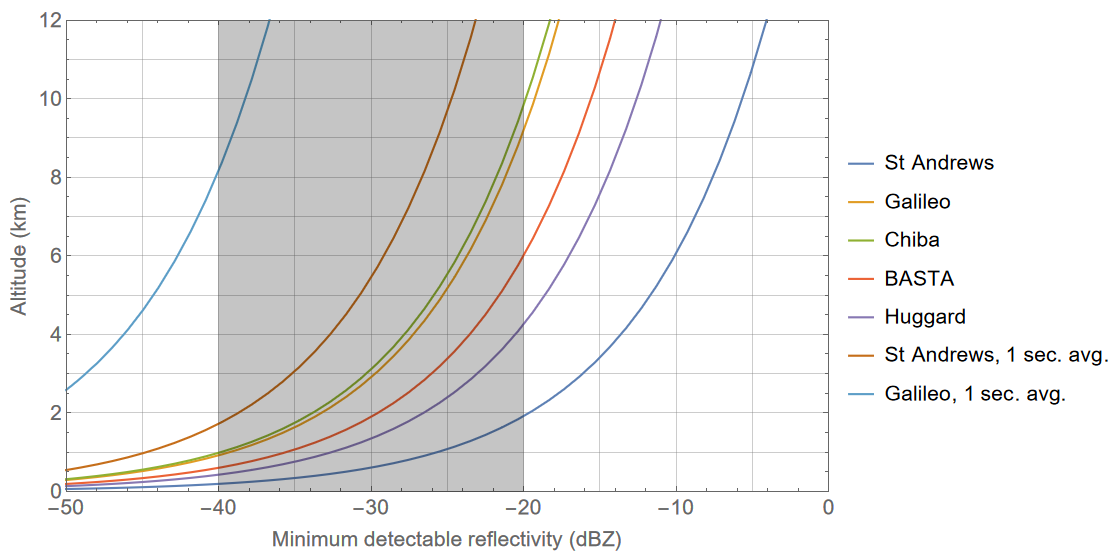
\includegraphics[width=\textwidth]{sensitivity-2}
	\caption{Predicted minimum detectable reflectivity curves using parameters for the radars described in Table \ref{tbl:RadarSystems}. Assumes a desired signal-to-noise ratio of \(1\), an ambient temperature of \SI{290}{\kelvin}, and \(\abs{K}^2 = 0.846\) which is appropriate for cloud particles in the water phase and an incident wavelength of \SI{3.2}{\milli\metre} (\SI{94}{\giga\hertz}).\supercite{ComplexIndexOfRefraction} The main region of interest for cloud radars is highlighted in grey. The \SI{1}{\second} non-coherent averaging curves assumes a \(\sqrt{N}\) improvement to the signal-to-noise ratio, where \(N\) is the number of chirps averaged together. (Own work)}
	\label{fig:Sensitivity}
\end{figure}

\section{Project work}
The St Andrews radar software needs to be updated to allow for averaging, extraction of Doppler moments, and real-time output. Also, calibration and some outdoor testing needs to be performed, in particular assessing the effect of ambient temperature on radar performance.
\paragraph{Signal averaging.} Averaging of range profiles reduces noise and increases sensitivity to low reflectivity clouds such as thin cirrus. Figure \ref{fig:Sensitivity} shows that without averaging the radar will be unable to detect any clouds above \SI{2}{\kilo\metre}.
\paragraph{Doppler moments.} Extraction of Doppler moments provides meteorologists with further information on the microphysical processes behind cloud formation.
\paragraph{Real-time output.} Real-time saving in netCDF,\supercite{NetCDFFormat} a format widely used by meteorologists. This would allow for offline data processing. Most of the radars in Table \ref{tbl:RadarSystems} support exporting data in netCDF format.
\paragraph{Effect of ambient temperature.} Changes in ambient temperature could affect the radar performance. Solid-state devices are particularly vulnerable to thermal drift. Thermal sensors in the radar enclosure will record the ambient temperature over a long period of time which can be correlated to radar performance.
\paragraph{Cross-check results with disdrometer.} Time permitting, a disdrometer located next to the radar can be used to record the drop-size distribution while raining. From this, the expected reflectivity can be calculated and compared to the output from the radar.

\section{Conclusions}
This article provided an introduction to millimetre wave cloud profiling radar, covering the principes of range, velocity, and reflectivity measurement using FMCW-Doppler processing. A select few modern cloud profiling radars were compared by their sensitivity.
Cloud radars, particularly at \SI{94}{\giga\hertz}, will remain an invaluable tool in the study of clouds. Low-cost millimetre wave FMCW-Doppler radars could mean wider deployment of cloud radars, improving weather forecasts and climate models.

\printbibliography
\end{document}
